As shown in section \ref{sec:alg}, multi-view deconvolution relies on 3D image stack convolutions with large kernels. In order to iterate towards an efficient design of multi-view deconvolution, this section will discuss model implementations and their benchmarks on hardware introduced in section \ref{sec:hw}. All of the model systems use synthetic data which is validated after each run upon consistency where appropriate. If not stated otherwise, the synthetic data has been generated in steps of powers of 2 in each dimension, so that each benchmark was run on $64x64x64$, $128x64x64$, $128x128x64$, \dots, $1024x1024x1024$ shaped datasets if possible.

\subsection{Single FFT}

As the heart of the application are FFT, there performance on CPU and GPU should be compared. For this, the most simple setup is used.

\begin{lstlisting}[caption={Single FFT on synthetic data performed on CPU in pseudo-code based on the \fftw{} syntax.},label={lst:single_fft_cpu}]
stack_f32 synthetic_data;

fftwf_plan plan = fftw_plan_dft_r2c(3,
                                    synthetic_data.shape(),
                                    synthetic_data.ptr(),
                                    synthetic_data.ptr(),
                                    FFTW_MEASURE);
//start timing
fftwf_execute(plan)
//end timing
\end{lstlisting}

Listing \ref{lst:single_fft_cpu} gives an overview on the syntax required to execute a \fftw{} 3D FFT on spatial domain data and whose result is written back to the same memory location in the frequency domain (in-place transform). The application programming interface (API) requires plan to perform the transform operation. According to the documentation \cite{fftw_manual}, the plan allocates additional memory for structures required during FFT execution. This global variable hence exerts a software design force on all clients to be aware of this behavior. Moreover, plans should be reused in order to prevent unnecessary reallocations. The equivalent implementation to perform the FFT on the \gpu{} is given in listing \ref{lst:single_fft_gpu}.\newline

\begin{lstlisting}[caption={Single FFT on synthetic data performed on GPU in pseudo-code based on the \cufft{} syntax.},label={lst:single_fft_gpu}]
stack_f32 synthetic_data;
float* device_ptr = 0;
cudaMalloc(device_ptr, sizeof(float)*synthetic_data.size());
cudaMemcpy(device_ptr, synthetic_data.ptr() , sizeof(float)*synthetic_data.size(), cudaHostToDevice);

cufftHandle plan;
cufftPlan3d(&plan,synthetic_data.shape(0),synthetic_data.shape(1),synthetic_data.shape(2),CUFFT_R2C);

//start timing
cufftExecR2C(plan, device_ptr, device_ptr);
//end timing

cudaMemcpy(synthetic_data.ptr(), device_ptr , sizeof(float)*synthetic_data.size(), cudaDeviceToHost);
\end{lstlisting}

Clearly, the offload model of having \gpu{} memory being separate from \cpu{} memory requires a lot more syntax than for plain \cpu{} use cases. However, the \cufft{} API is similar in nature to \fftw{} except the more stringent procedural approach (no functions with return values, rather than functions operating on structs). As \texttt{cudaMemcpy} is used to transfer data from host to device and back, this implementation is internally synchronized.\newline

\begin{figure}[h]
  \centering
  \hfill
  \begin{subfigure}[b]{0.45\textwidth}
    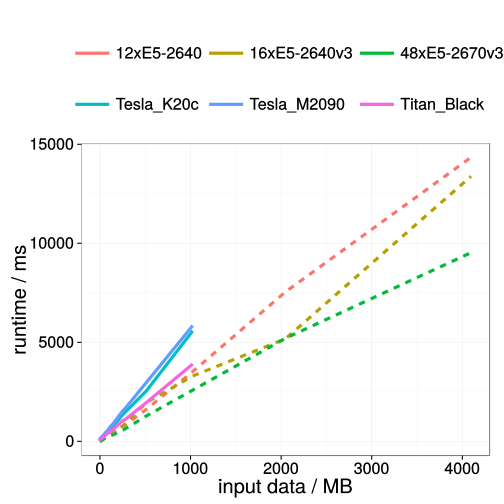
\includegraphics[width=\textwidth]{plots/synced_gpu_runtime}
    \caption{CUDA runtime}
    \label{fig:single_fft_runtime}
  \end{subfigure}%
  \hfill
  \begin{subfigure}[b]{0.45\textwidth}
    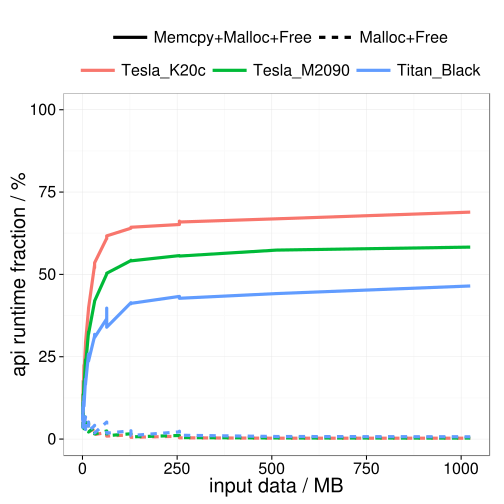
\includegraphics[width=\textwidth]{plots/synced_gpu_api_fraction}
    \caption{CUDA API fraction}
    \label{fig:single_fft_api_fraction}
  \end{subfigure}
  \hfill
  \caption{Runtimes for single 3D FFT on synthetic data on \cpu{} with \fftw{} and on \gpu{} with \cufft{} (left, \ref{fig:single_fft_runtime}) and API time fraction of runtime dedicated to data (de-)allocation and/or data transfer (right, \ref{fig:single_fft_api_fraction}).}
  \label{fig:rt_single_fft}
\end{figure}

Figure \ref{fig:rt_single_fft} illustrates the runtime budget of an FFT transformation for different input data performed on multi-core \cpu{}s or on \gpu{}s. Subfigure \ref{fig:single_fft_runtime} shows a linear rise in runtime with increasing size of input data. This is the behaviour expected from considerations of equation \ref{eq:fft_convol_complexity}. Due to the larger memory available on \cpu{}s, they are able to handle bigger data sets than \gpu{}s.\\

For the execution on a \gpu{}, it is interesting to observe what fraction of this runtime is invested in data transfers. Figure \ref{fig:single_fft_api_fraction} hints to $\unit[50-70]{\%}$ of the total runtime is dedicated to data transfers. It is interesting to see how the \gpu{} that supports PCI Express Gen3 clearly dedicates less time to memory transfers than the other modesl. \\

The API fraction measurements have been performed with \texttt{nvprof} called as in:\newline
\begin{center}
  \texttt{nvprof --normalized-time-unit ms --print-gpu-summary --print-api-summary --print-summary --profile-from-start off}\newline
\end{center}

Firgure \ref{fig:single_fft_api_fraction} implies, that if data transfer can be hidden or accelerated, this would be beneficial for the \gpu{} based algorithm to accelerate in comparions to the \cpu{} implementation.

\clearpage
\subsection{Batched FFTs}
As the transform of a single data volume is of minimal use for the application at hand, the next step is to study the transform of a sequence of image stacks with fixed sizes.

\begin{lstlisting}[caption={Batched FFT on synthetic data performed on CPU in pseudo-code based on the \fftw{} syntax.},label={lst:batched_fft_cpu}]
stack_f32 synthetic_data[n_view];

fftwf_plan plan = fftw_plan_dft_r2c(3,
                                    synthetic_data[0].shape(),
                                    synthetic_data[0].ptr(),
                                    synthetic_data[0].ptr(),
                                    FFTW_MEASURE);
//start timing
for ( v : n_view )
  fftwf_execute_dft_r2c(plan, 
                        synthetic_data[v].ptr(),
                        synthetic_data[v].ptr());
//end timing
\end{lstlisting}

As listing \ref{lst:batched_fft_cpu} illustrates, plan reuse is performed and \fftw{} is called with the \texttt{FFTW\_MEASURE}. During plan creation, the \fftw{} library tries to find the best FFT implementation for the given buffer shape. \texttt{FFTW\_MEASURE} guarantees a next-to-optimal solution. The GPU implementation at this point already requires a complex orchestration of memory transfer streams and execution.

\begin{figure}[h]
  \centering

  \begin{subfigure}[b]{0.9\textwidth}
    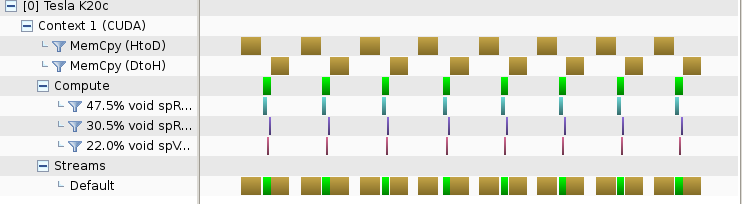
\includegraphics[width=\textwidth]{img/bench_gpu_many_nd_fft_sync_narrow}
    \caption{synchronized transform}
    \label{fig:batched_fft_sync}
  \end{subfigure}%

  \begin{subfigure}[b]{0.9\textwidth}
    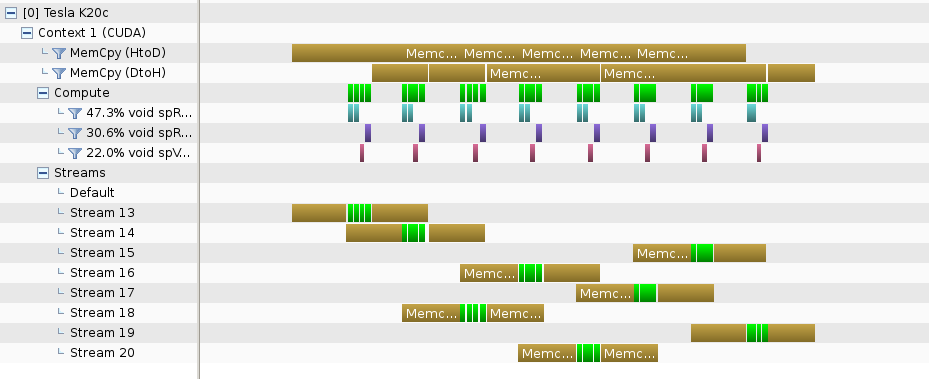
\includegraphics[width=\textwidth]{img/bench_gpu_many_nd_fft_async_narrow}
    \caption{asynchronous transform}
    \label{fig:batched_fft_async}
  \end{subfigure}%

  \begin{subfigure}[b]{0.9\textwidth}
    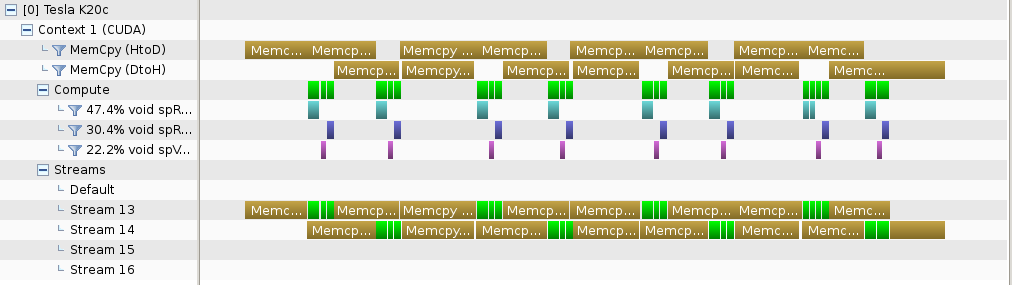
\includegraphics[width=\textwidth]{img/bench_gpu_many_nd_fft_async2plans_narrow}
    \caption{asynchronous transform with 2 streams}
    \label{fig:batched_fft_async2plans}
  \end{subfigure}%

  \caption{\texttt{nvprof} screenshot of batched FFT transforms.}
  \label{fig:nvprof_batched_fft}
\end{figure}

Figure \ref{fig:nvprof_batched_fft} illustrates possible advantages and disadvantages of the applied techniques. As the documentation of the corresponding code for figure \ref{fig:nvprof_batched_fft} would be rather long, the interested reader is deferred to \texttt{bench\_gpu\_many\_nd\_fft.cu} of the \lmvn{} benchmark suite available through \cite{lmvn_repo}. 

\begin{lstlisting}[caption={Asynchronous Batched FFT on synthetic data performed on GPU in pseudo-code based on the \cufft{} syntax.},label={lst:batched_fft_gpu_async2plans}]
stack_f32 synthetic_data[n_view];
cudaEvent_t stream_events[n_view];
fftwf_plan plans[2];
cudaStream_t streams[2];
float* d_buffer[2];
// ... initialize 

//start timing
for ( v : n_view ){
  cudaMemcpyAsync(synthetic_data[v] -> d_buffer[v \% 2],streams[v \% 2]);
  cudaEventRecord(stream_events[v],streams[v \% 2]);
  cudaStreamWaitEvent(streams[v \% 2],stream_events[v - 1]);
  cufftExecR2C(plans[v \% 2], d_buffer[v \% 2]) // on stream d_buffer[v \% 2]
  cudaMemcpyAsync(d_buffer[v \% 2] -> synthetic_data[v],streams[v \% 2]);
}
cudaDeviceSynchronize();
//end timing

//clean-up
\end{lstlisting}


What however becomes clear is that synchronous (figure \ref{fig:batched_fft_sync}) are not beneficial as data transfers to the \gpu{} are performed sequentially. Asynchronous transfers using the same number of streams as there are image stacks (figure \ref{fig:batched_fft_async}) are also not performant (mostly due to the lack of copy engines). But if the number of transfer streams correlates with the number of copy engines the \gpu{} offers, data transfers and computations can be overlaid to some higher extent and runtime benefits can be obtained (figure \ref{fig:batched_fft_async2plans}). Besides the ones just discussed, other host-device data transfer methods were benchmarked. 
For example, mapped memory usage (buffers are marked by \texttt{cudaHostRegister} and their device pointer is obtained through \texttt{cudaHostGetDevicePointer}) and managed unified memory (all data is allocated by \texttt{cudaMallocManaged}) have been implemented. The results for ``managed'' memory usage are not shown here because time measurements did not correlated at all with the measurements obtained in \texttt{nvprof}. Before drawing wrong conclusions, the data is not discussed at all. 

\begin{figure}[h]
  \centering
  \hfill
  \begin{subfigure}[b]{0.45\textwidth}
    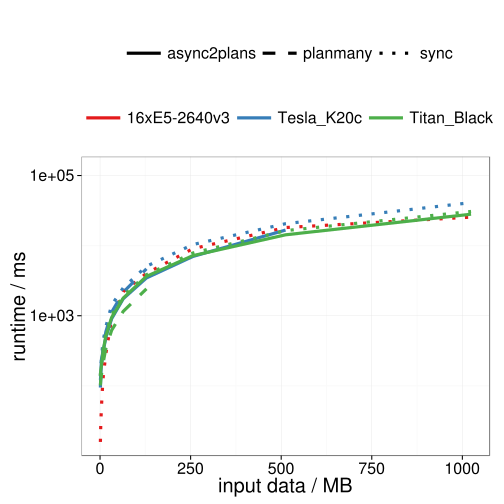
\includegraphics[width=\textwidth]{plots/batched_cgpu_runtime}
    \caption{CUDA runtime}
    \label{fig:batched_fft_runtime}
  \end{subfigure}%
  \hfill
  \begin{subfigure}[b]{0.45\textwidth}
    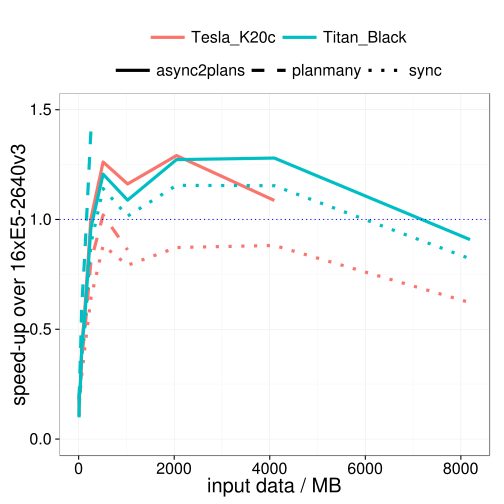
\includegraphics[width=\textwidth]{plots/batched_gpu_speed_up}
    \caption{\gpu{} speed-up versus \cpu{}}
    \label{fig:batched_fft_speed_up}
  \end{subfigure}
  \hfill
  \caption{Runtimes for batched 3D FFT on synthetic data on \cpu{} with \fftw{} and on \gpu{} with \cufft{} (left, \ref{fig:single_fft_runtime}) and the relative speed-up of the asynchronous \gpu{} implementation using 2 streams (see figure \ref{fig:batched_fft_async2plans}) compared to the multi-core \cpu{} implementation (right, \ref{fig:batched_fft_speed_up})}
  \label{fig:rt_batched_fft}
\end{figure}


Firgure \ref{fig:rt_batched_fft} shows that the implementation using ``mapped'' memory chosen for this benchmark is clearly very slow. The synchronized implementation is on par with the \cpu{} implementation for data volumes of $\unit[150]{MB}$ and less. Above this threshold, the multi-core implementation is more performant. As emphasized by figure \ref{fig:batched_fft_speed_up}, given an input data volume of $\unit[50-250]{MB}$, this implementation is faster than the \cpu{} implementation. The situation depends on the \gpu{} model. This is due to the fact that both the GeForce Titan Black and the Tesla M2090 do only contain 1 copy engine. The device is henceforth forced to serialize asynchronous data transfers and kernel execution.\newline

It must be noted at this point, as the application at hand (see listing \ref{lst:java_implementation}) is applied to large data sets, the use of \texttt{cufftPlanMany} is prohibitive. At the time of writing, a subsequent call to \texttt{cufftExecR2C} on a plan thus created must retain all input/output data on device. Using \texttt{cufftPlanMany} in the context of figure \ref{fig:rt_batched_fft} may be considered an important reference benchmark.

\subsection{Batched Convolutions}


\subsection{Library Implementation}

